\documentclass[12pt,a4paper,oneside]{article}
% nagyon sok kép esetén meggyorsítható a fordítás a draft móddal
% \documentclass[12pt,a4paper,oneside,draft]{report}
% ekkor a képek nem renderelődnek ki, csak placeholder lesz mérethelyesen
\usepackage[utf8]{inputenc} % mindenképp maradjon az utf-8 kódolás
\usepackage[magyar]{babel}
\usepackage[T1]{fontenc}
\usepackage{amsmath}
\usepackage{amsfonts}
\usepackage{amssymb}
\usepackage{graphicx} % grafikus elemek, képek berakásához
%\usepackage{epsfig} % eps importáláshoz
\usepackage{listings}
\usepackage{sectsty}
\usepackage{enumerate}
\usepackage{siunitx} % ezzel lehet hivatalosan megformázni: szám + mértékegység
\usepackage{lastpage}
\usepackage{setspace}
\usepackage{hyperref} % PDF hivatkozásokhoz kell
\usepackage[hang]{caption}
\usepackage{titling} % a title, author parancsok szabad használatához
\usepackage{xcolor}
\usepackage{multicol}
\usepackage[hyphenbreaks]{breakurl}


\pagenumbering{arabic}

\definecolor{rosewood}{rgb}{0.6, 0.0, 0.04}
\definecolor{indigo(dye)}{rgb}{0.0, 0.25, 0.42}

\usepackage[left=25mm,right=25mm,top=20mm,bottom=25mm]{geometry}\pagestyle{plain}

%\singlespacing
\onehalfspacing

\def\UrlBreaks{\do\/\do-\do_}

\hypersetup
{
  	colorlinks,
  	citecolor=blue,
 	linkcolor=rosewood,
  	urlcolor=indigo(dye)
}
\title{Nem optikai elven működő \\ kvantum véletlenszám generátorok} 
\author{Szilágyi Gábor}
\date{\today}
\setlength{\unitlength}{1cm} % fix unit

\begin{document}
\maketitle
\section*{Bevezetés}
A véletlen számokat számos területen használnak. Ide tartozik a kriptográfia, ezen belül például az Internet Of Things (IoT) eszközök közötti kommunikáció, a digitális aláírások, a digitális szolgáltatások felhasználóinak azonosítása, az egyszerhasználatos kulcsok (One-Time Pad) generálása, vagy a banki tranzakciók adminisztrációja. Bizonyos szimulációs eljárásoknál -- elsősorban a Monte-Carlo módszernél -- a szimulációs eredmények helyessége a felhasznált véletlen számok véletlenszerűségén nyugszik. Választások lebonyolításánál és szerencsejátékoknál is fontos a felhasznált véletlen számok kompromittálatlansága, itt elsősorban sorsolásra használják fel a véletlen számokat. Mesterséges intelligenciák evolúciójánál a túlélő példányok kiválasztása, tulajdonságaik összekeverése, valamint a mutációik is fontos, hogy teljesen véletlenszerűek legyenek. Neurális hálóknál az élek véletlenszerű súlyozása is véletlen számokat igényel. Végül, de nem utolsósorban a kriptovalutákat kezelő infrastruktúrákban is fontos szerepe van a véletlen számoknak.
\par
A fenti felsorolás messze nem kimerítő, ebből is látszik, hogy a véletlen számok nagy hatással vannak a mai világ működésére. A felhasznált véletlen számok megjósolhatóságának súlyos következményei lehetnek, mert sok esetben teljesen meghiúsítják az őket felhasználó alkalmazások működését, ami nagy veszteségeket okozhat. Ilyen esetekre néhány példa a közelmúltból \cite{altalanos-random}:
\begin{itemize}
	\item 2010-ben a Sony PlayStation 3 játékkonzol 77 millió felhasználójának adatait ellopták a támadók. A támadáshoz a cég ECDSA (Elliptic Curve Digital Signatura Algorithm) implementációjának hibáját használták ki, ami miatt ugyanazt a számot többször használta fel az algoritmus a felhasználók azonosításához \cite{sony}.
	\item 2012-ban két kutatócsoport több olyan RSA titkosítási kulcsot hozott napvilágra, amiket addig aktívan használtak az interneten biztonságosnak hitt kulcsként, de feltörhetőek voltak amiatt, hogy nem megfelelő véletlenszám generátort használtak a kulcsok generálásakor \cite{bad-rsa}.
	\item 2015-ben 18866 Bitcoint loptak el a Bitstamp kriptovaluta tőzsdén, ami az ott forgalomban lévő kriptopénz 12\%-át jelentette ekkor. A támadás kapcsán a véletlen számok hibás generálásának kihasználására utaló nyomok kerültek napvilágra \cite{bitstamp}.
\end{itemize}
\section*{A véletlenszerűség definiálása}
Ugyan elég jól körül lehet írni a valódi véletlent és fel tudunk sorolni olyan tulajdonságokat, amik biztosan igazak egy véletlenszerűen előállított bitsorozatra, de a matematika mai eszköztárával nem sikerült általános, formális definíciót találni a valódi véletlenre.
\par
A valódi véletlenszerűség eldöntéséhez a legjobb, amit tehetünk, az a különböző tesztek lefuttatása a vizsgált bitsorozaton. Ezek semmilyen véges hosszú bitsorozatra alkalmazva nem tudnak egyértelmű választ adni arra a kérdésre, hogy az valóban véletlen-e, de a segítségükkel legalább azt el lehet dönteni, hogy a generálás módszere a vizsgált szempontokból mennyire áll közel az igazi véletlenhez.
\par
Matematikailag nehezen kezelhető a tökéltes véletlenszerűség, de vannak olyan fizikai folyamatok, amelyek a tudomány mai állása szerint teljesen kiszámíthatatlanok, emiatt megfelelnek a tökéletes véletlenszerűségről alkotott elképzeléseknek. Az ilyen fizikai folyamatok a kvantumfizika területén keresendőek, tehát kis méretskálán működnek, nagyságrendileg az egyedüli részecske (általában atom, elektron vagy foton) szintjén. Több ilyen folyamat is ismert, a rájuk épülő véletlenszám-generátorok kivitelezhetősége változó. Az említett fizikai folyamatok jó része optikai alapú, vagyis fotonok véletlenszerű viselkedésére épül, emiatt alapvetően két csoportba szokták osztani: optikai- és nem optikai folyamatokra. Ez a tanulmány az utóbbi csoportba tartozó folyamatokra építő véletlenszám generátorokkal foglalkozik.
\par
A kvantum folyamatok kimenetele lehet teljesen kiszámíthatatlan, de ha egy ilyen folyamatot felhasználó véletlenszám generátort realizálunk, akkor az valamilyen mértékben ,,szennyezni'' fogja a kvantum folyamatra vonatkozó mérési eredményeket valamilyen determinisztikus zajjal. Emiatt nyer értelmet a véletlenszám generátorok kimenetének osztályozása aszerint, hogy mennyire véletlenszerűek.
\par
A véletlenszám generátorok minőségi osztályozására előre definiált tesztcsomagokat szokás használni, amelyek több szempontból ellenőrzik a generátor viselkedését. Egy egyszerűbb szempont az ismétlődő minták keresése a generált bitsorozatban. Két véletlenszám generátorok működésének ellenőrzésére használt tesztcsomag a NIST SP 800-22 NIST \cite{nist1} és a SP 800-90B \cite{nist2} (NIST -- National Institute of Science and Technology).
\section*{Véletlenszám generátorok}
Egy véletlenszám generátornak két paramétere kritikus, az egyik a számok megjósolhatatlanságának minősége, a másik a generálás bitsebessége.
\par
Bizonyos alkalmazásoknál a két paraméter közül nagy bitsebesség sokkal fontosabb, ekkor megengedhető lehet olyan véletlenszám generátor használata, ami valójában determinisztikus módon hozza létre a kimeneti bitsorozatát, ezek a pszeudo-véletlen generátorok, amelyek gyakran (de nem feltétlenül) szoftveresen vannak implementálva. A pszeudo-véletlenszám generátorok hátránya, hogy a kimeneti bitsorozatuk különböző módokon előre kiszámítható lehet, emiatt nem felelnek meg a tökéletes véletlenszerűség kritériumainak.
\par
Ahol a generált bitsorozat ,,minősége'' fontos, ott olyan fizikai folyamatot érdemes alapul venni a bitek előállításához, ami valóban kiszámíthatatlan. Az ilyen folyamatok a klasszikus fizika helyett a kvantumfizika területén keresendőek. A kvantum folyamatok használatának egyik előnye, hogy a véletlen számokkal szemben támasztott követelményeknek automatikusan megfelelnek. A kvantumszámítógépek fejlesztése az elmúlt években olyan szintre jutott, hogy a determinisztikus úton előállított véletlen bitsorozatokat már az a veszély fenyegeti, hogy még ha ugyan klasszikus számítógépekkel nem is, de kvantumszámítógépek segítségével megjósolhatóak lehetnek. Abban rejlik a kvantum véletlenszám generátorok másik előnye, hogy a segítségükkel előállított bitsorozatok elméletileg kvantumszámítógépek segítségével is megjósolhatatlanok.
\par
Létezik a fent leírt végletek közötti kompromisszumos megoldás, ami abban áll, hogy egy relatíve lassú kvantum véletlenszám generátor (entrópiaforrás -- entropy source) kimenetét egy determinisztikus algoritmusban kiindulási változóként (random seed) használjuk. A determinisztikus algoritmus a saját kimenetén egy a bemenetihez képest sokszoros hosszú bitsorozatot generál, de ez az új bitsorozat az algoritmus paraméterei és a kiindulási változó ismeretében teljesen reprodukálható. Ezért ezzel a megoldással nem minden esetben lehet kiváltani a teljesen kvantum generátort.
\par
A fenti okok miatt egyre nő és egyre több alkalmazási területet érint a kvantum folyamatokon alapuló véletlenszám generátorok iránti igény.
\section*{Radioaktív bomlás alapú generátorok}
A  radioaktív bomlási folyamatok instabil atommagokban játszódnak le, amik úgy veszítenek energiát a folyamat során, hogy valamilyen részecskét (részecskéket) bocsátanak ki és más össztételű atommaggá alakulnak közben. Ezeknek a bomlási folyamatoknak a bekövetkezési ideje az előre teljesen meghatározhatatlan és kívülről befolyásolhatatlan. Ezek a folyamatok a radioaktív izotóp felezési idejével ($\lambda$) jellemezhetőek, ami azt az időtartamot jelenti, ami alatt pontosan 1/2 valószínűséggel következik be egy adott atommagban a bomlási folyamat. Ha makroszkopikus mennyiséget veszünk egy ilyen radioaktív izotópból, akkor abban az elbomlás nélkül megmaradt atomok száma exponenciálisan, gyakorlatilag folyamatosan csökken -- találóan felezési időnként feleződik.
\par
A radioaktív bomlások különböző kisugárzott részecskékkel járhatnak, a különböző bomlási folyamatok jellemzőek az egyes instabil izotópokra. A kibocsátott részecskék között lehetnek neutrínók, pozitronok, valamint hélium atommagnál nehezebb atommagok is, de a gyakoribb kisugárzott részecsketípusok az alfa-, béta- és gamma-részecskék.
\begin{itemize}
	\item Az alfa-részecske egy hélium atommag. Az alfa-sugárzás relatíve könnyen árnyékolható, erre egy papírlap is képes. A nagy roncsoló hatása miatt veszélyes az élőlényekre.
	\item A béta-részecske egy elektron. Megkülönböztetnek $\beta^-$ és $\beta^+$ sugárzást, ezek elektron és pozitron (antielektron) sugárzást jelentenek sorrendben. A béta-sugárzás valamivel nehezebben árnyékolható, mint az alfa, de még mindig nem túl nehezen -- például egy vékony alumíniumlemez is jó árnyékoló hatású.
	\item A gamma részecske egy nagyenergiájú foton, ami nehezen árnyékolható, de emellett nagy roncsoló hatású is, ezek kombinációja kifjezetten veszélyessé és nehezen kezelhetővé teszi. A gamma-sugárzás elleni árnyékolás körülményes, például egy vastag ólomréteg tud hatásos lenni ebben a tekintetben.
\end{itemize}
\par
Radioaktív anyagok felhasználásával elsősorban olyan véletlenszám-generátor készíthető, ami az egymás után kisugárzott részecskék detekciója között eltelt idő alapján számolja ki a véletlen biteket. A mért időintervallumok nyers számértéke közel sem egyenletes eloszlású, ami ideális lenne a véletlen bitek generálásához. Egy jobban használható megközelítésben, a detekciók közötti időt nagyon pontosan megmérjük, majd a mért számérték legkisebb helyiértékű bitjeit használjuk véletlenszerűen generált bitekként. Ha a legkisebb helyiértékű biteken ábrázolható időtartam elég kicsi a detekciók között átlagosan eltelt időhöz képest, akkor ezekből a bitekből alkotott számok eloszlása már jó közelítéssel egyenletes.
\par
\begin{figure}[ht!]
	\centering
	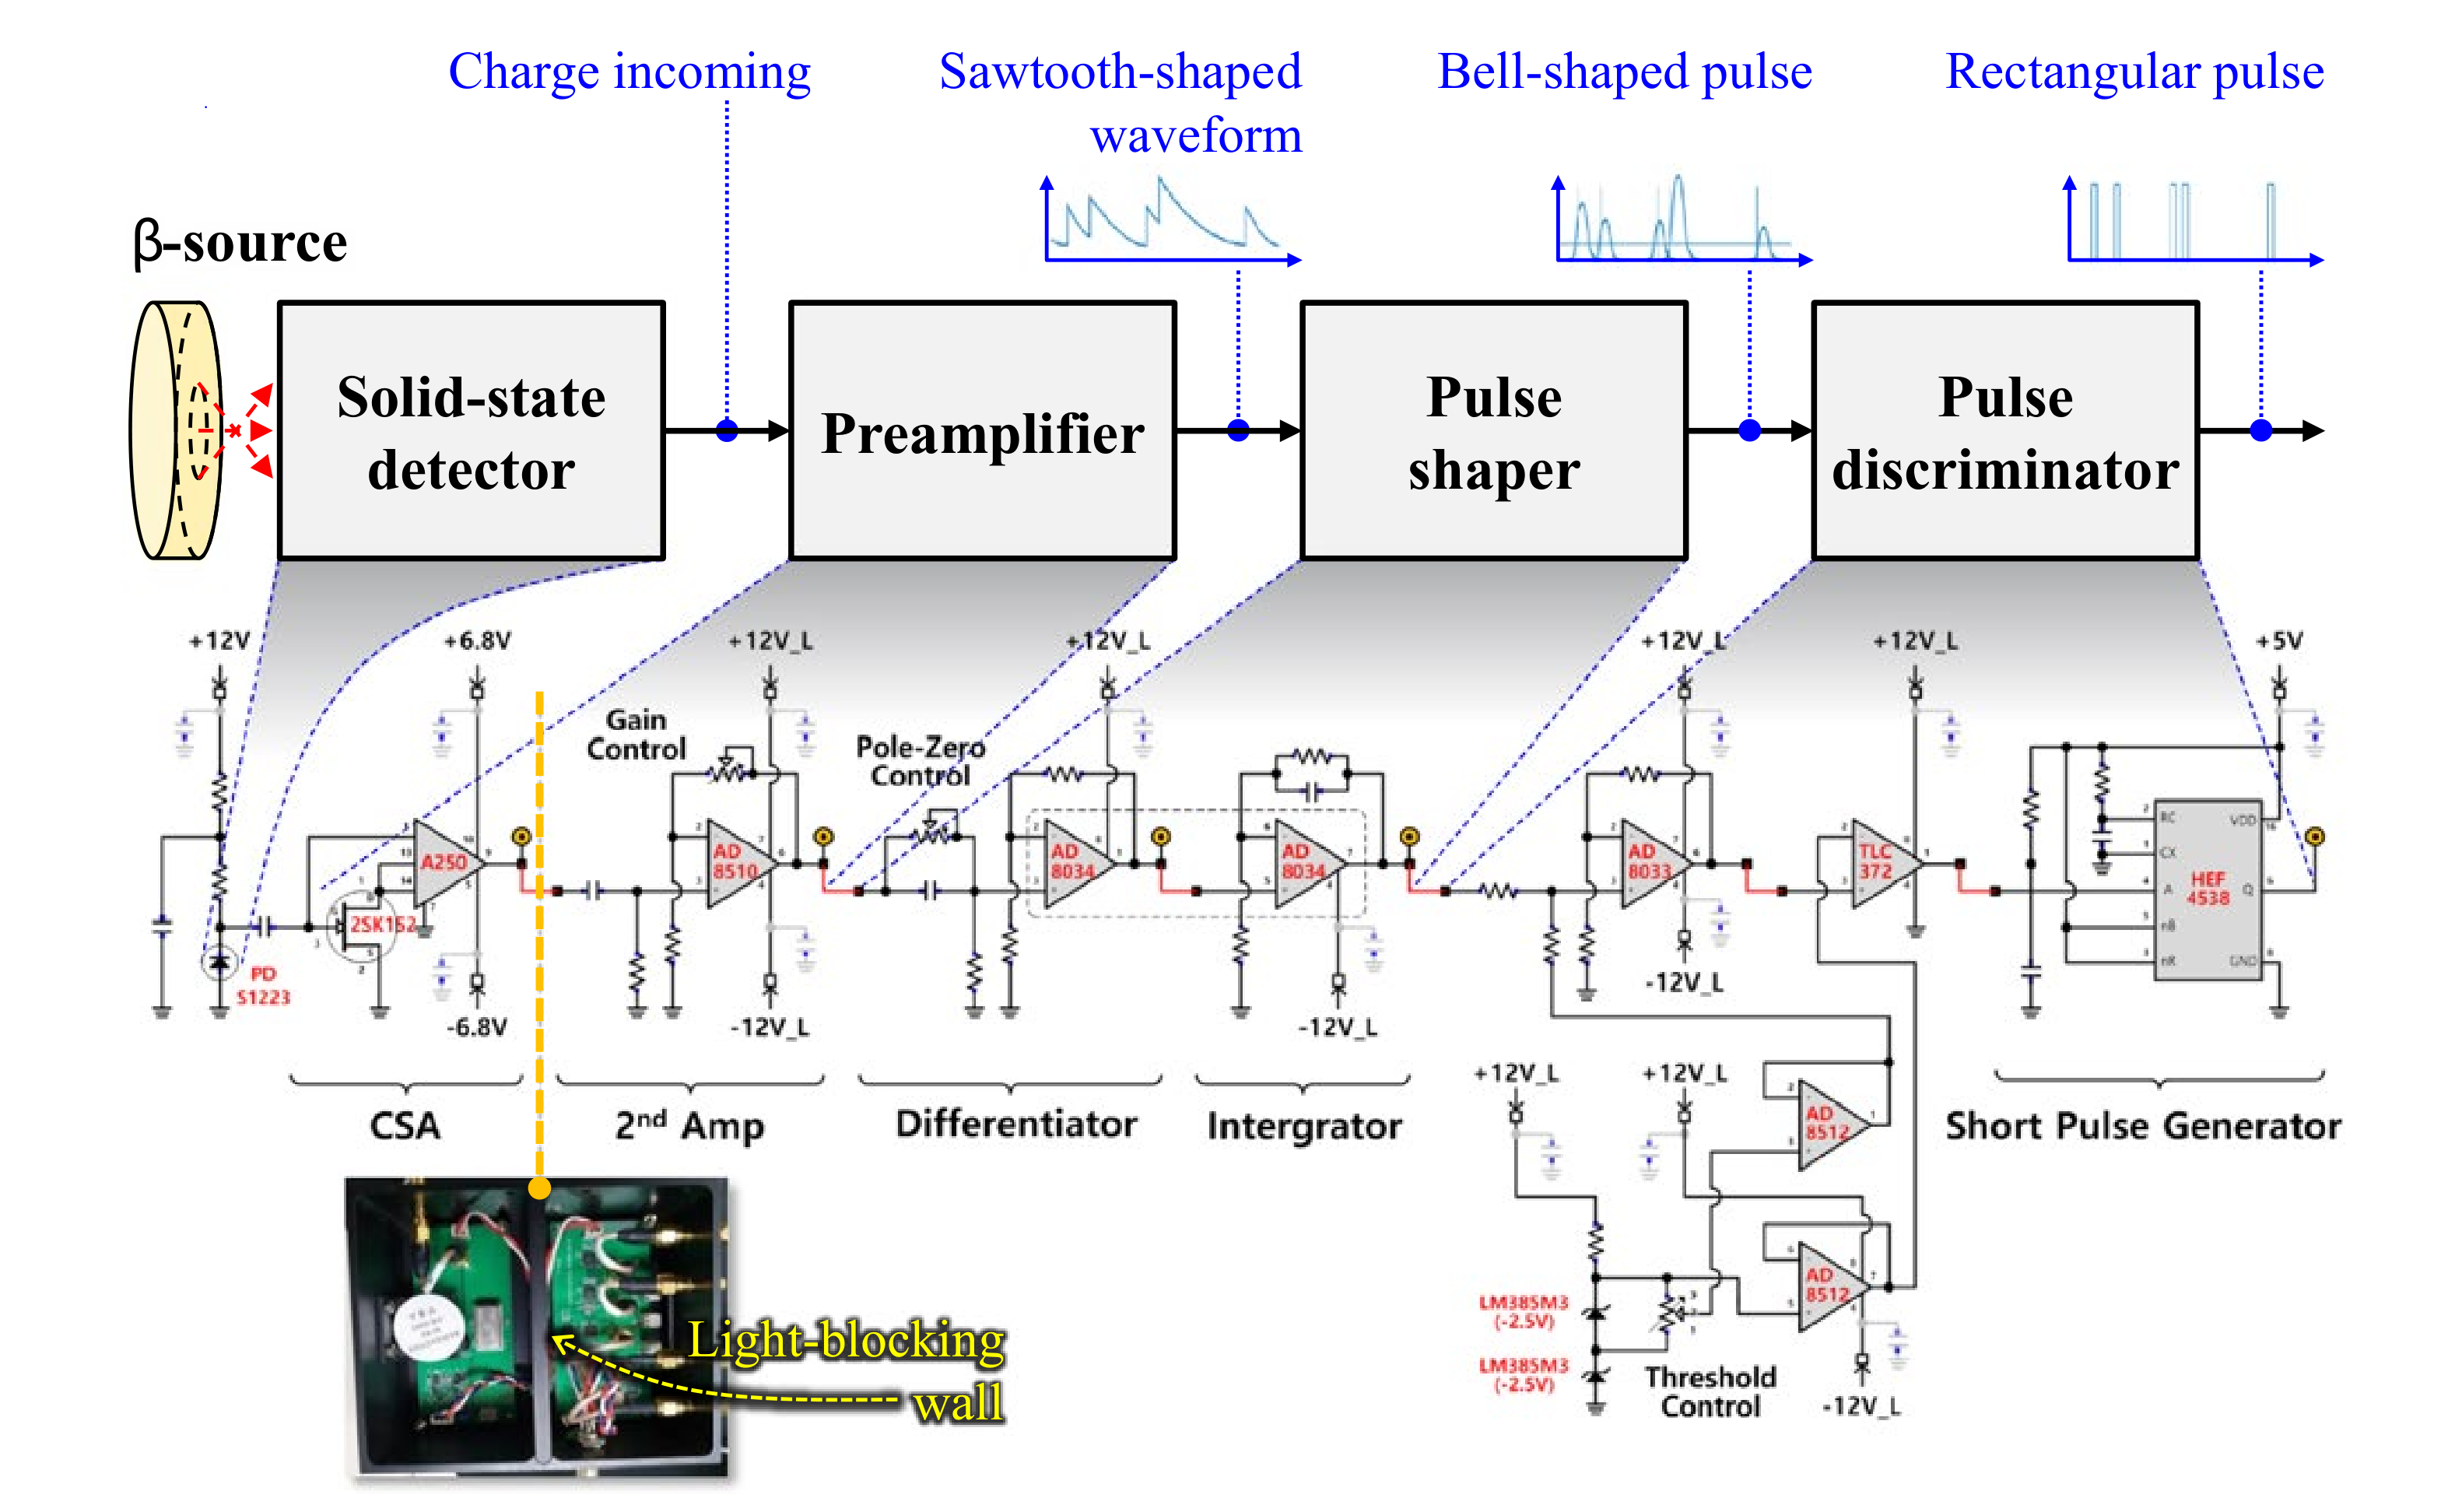
\includegraphics[width=0.7\textwidth]{beta1.png}
\end{figure}
A fent leírt elven működő véletlenszám generátort terveztek (és fejlesztenek) egy az \textit{ETRI Journal} c. folyóiratban megjelent cikk szerzői \cite{beta}. Ez a véletlenszám generálási módszer önmagában nem újdonság, de a cikkben egy olyan megvalósításról van szó, ami a kvantum véletlenszám generálás legtöbb hátulütőjét ki tudja küszöbölni.

A cikkben leírt megvalósítás az IoT alkalmazásokat célozza, amik a különböző titkosítási protokollokhoz használnának véletlen számokat, de itt fontos a kis méret, az alacsony fogyasztás és a felhasználó egészségére jelentett veszély mértéke is. A tervezett generátor tisztán béta-sugárzó nikkel-izotópot használ sugárzó forrásnak. Azért esett a választásuk erre az anyagra, mert a tisztán béta-sugárzás miatt az eszköz könnyen leárnyékolható, valamint viszonylag nagy sugárzásérték is egészségügyileg engedélyezett ennél a konkrét izotópnál, ami gyakori részecskedetekciókat, ezáltal nagy bitsebességet eredményez.
\par
A cikkben a szerzők részletezik az eszköz különböző, személyreszabott igényekre való méretezésének lehetőségeit, valamint a detekciót végző áramkör felépítését és működését. A méretezéssel a fogyasztás, a fizikai kiterjedés és a bitsebesség közötti egyensúlyt lehet megtalálni különböző alkalmazások által támasztott igényeket is potenciálisan kielégítve ezzel.
\par
\begin{figure}[h!]
	\centering
	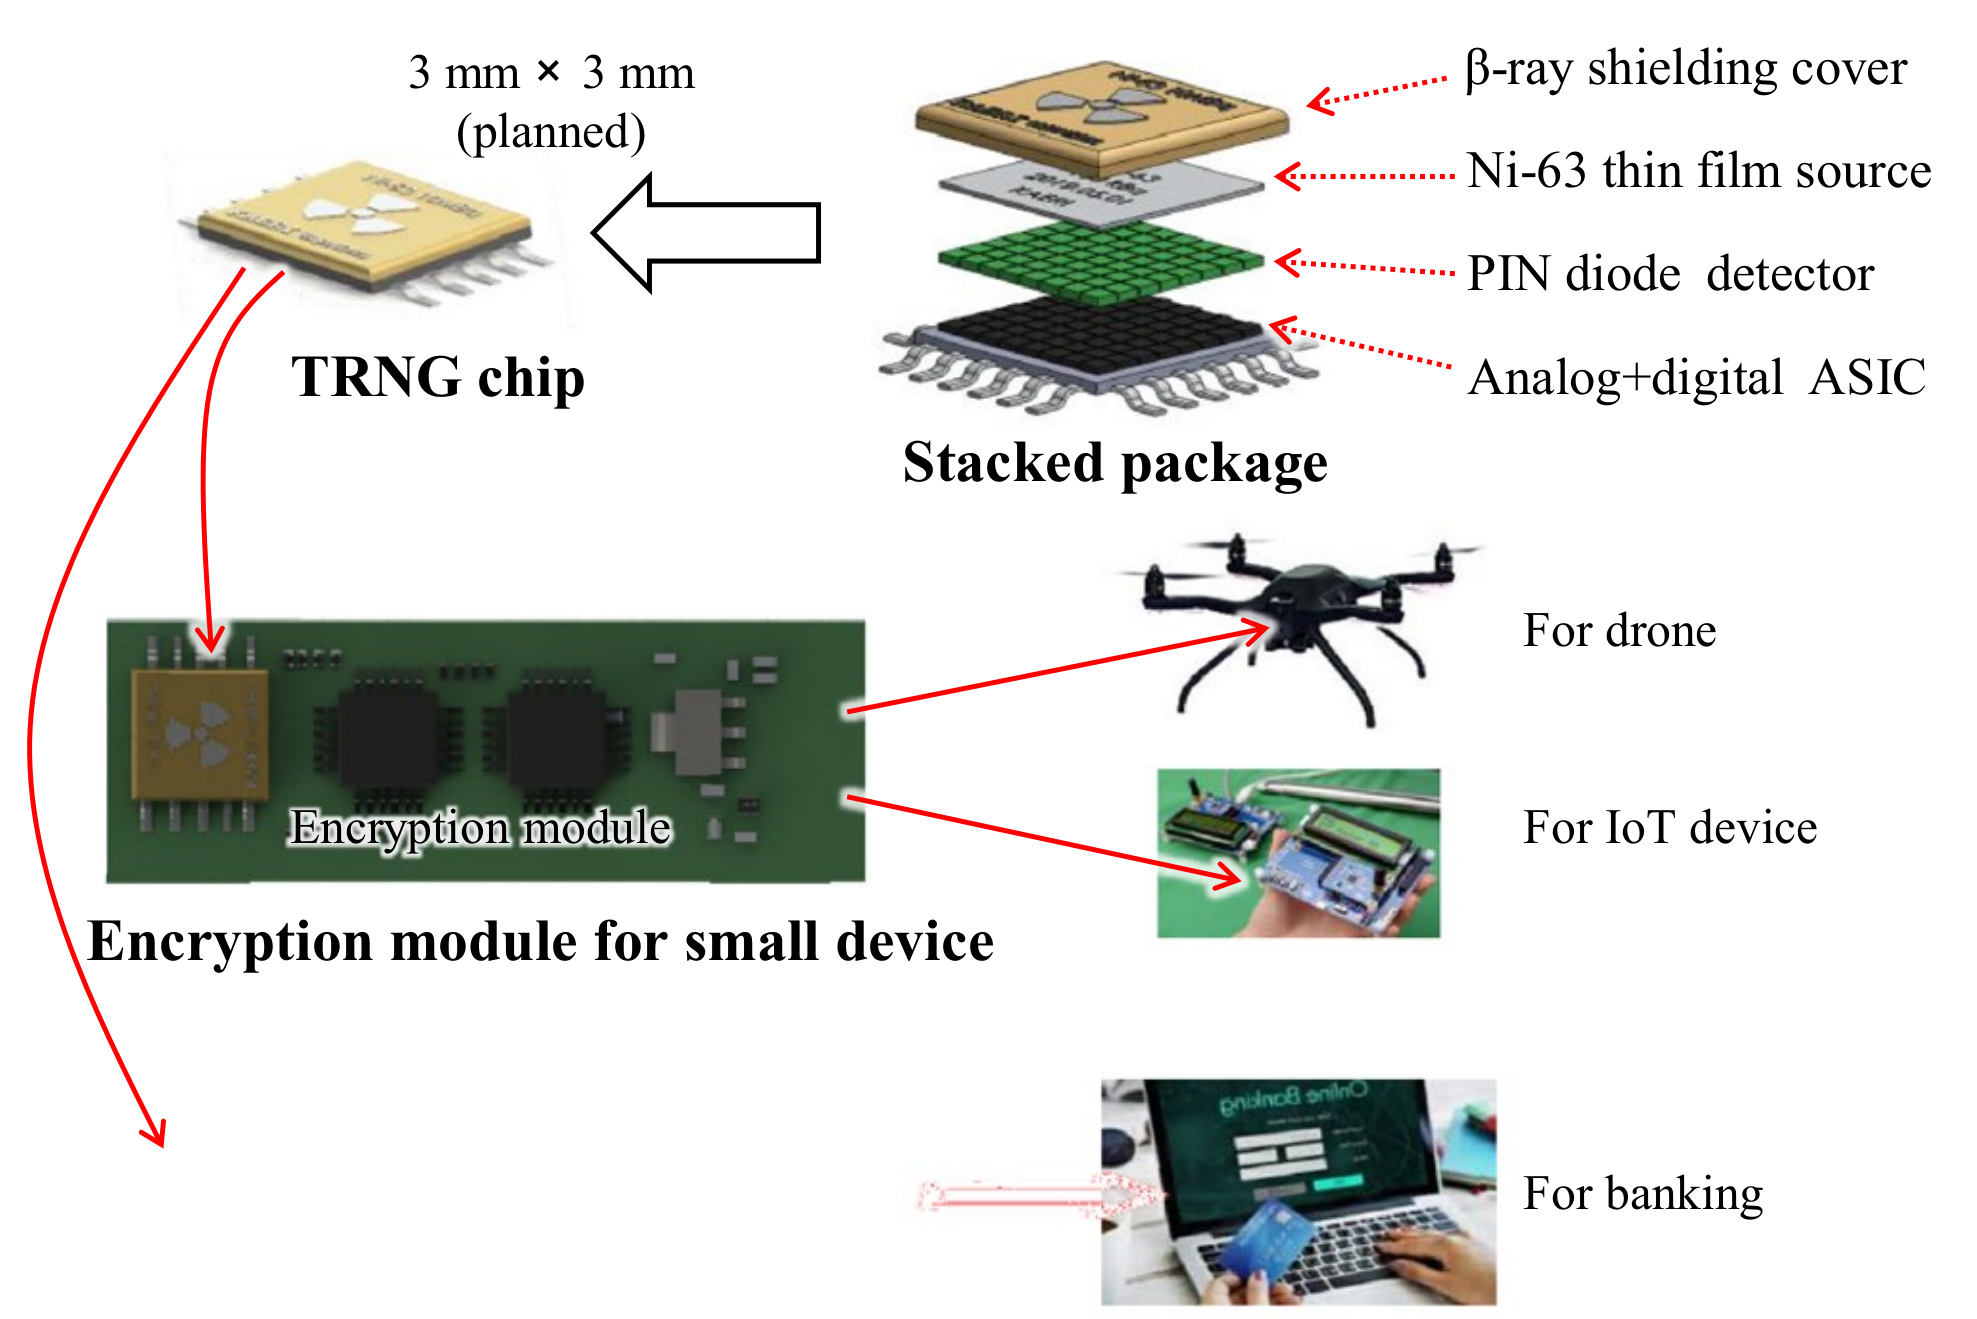
\includegraphics[width=0.7\textwidth]{beta2.png}
\end{figure}
A béta-részecskék detekciójához fordított előfeszítésű PIN diódákat használnak fel. Ezek a diódák minél nagyobb méretűek, annál több sugárzást lehet velük detektálni, de cserébe a méretükkel együtt megnő a rajtuk mérhető zaj is, ami a detekcióhoz szükséges minimális részecskeenergiát növeli. Emiatt a szerzők egy dióda-mátrixot használnak a nagyobb detekciós sebesség elérése érdekében.
\par
Egy kibocsájtott részecske detektálásának valószínűségét érdemes minél nagyobb szintre hozni a kialakított struktúrával, mert a nagyobb detekciós valószínűség adott sugárzási intenzitás mellett gyakoribb detekciót és ezáltal nagyobb maximális bitsebességet jelent. A sugárzó anyag által kibocsájtott részecskék energiája nem pontosan meghatározott, de az adott sugárzó anyagra jellemző eloszlású. A részecskék egy része olyan kis energiájú, hogy a detektor PIN-diódájának zajszintjéből nem kivehető az általa keltett jel, emiatt ezek nem detektálhatóak. Ha egy béta-részecske nem a detektor felé sugárzódik ki, akkor eleve 0 a detekció esélye. Ezen kívül ha a sugárzó anyag tömbjének feszínétől távol keletkezik a részecske, akkor ebből a tömbből való kijutás alatt is energiát veszít, amivel könnyen a detekciós küszöb alá kerülhet az energiája. Ezeknek a hatásoknak a kinimalizálására a sugárzó anyagot egy vékony lap formájában tartalmazza a generátor, aminek az egyik oldalát teljesen lefedve helyezkedik el közvetlenül alatta a detektor. Ezáltal a részecskék keletkezési helyének a sugárzó anyag felszínétől mért távolsága relatíve kicsi az össz térfogathoz viszonyítva, a lapos kialakítás miatt a kisugárzódás iránya miatti detekciócsökkenés elvileg csak 50\% körüli.
\par
Összességében körülbelül a kibocsájtott béta-részecskék 3\%-a detektálható a leírt elrendezéssel anélkül, hogy determinisztikus zaj által okozott hamis detekciók meghamisítsák a generált bitsorozatot. Ezáltal a sugárzás egészségügyi határértékeinek betartásával több Mbit/s bitsebesség érhető el a tervezett készülékkel.
\par
Összegzésként elmondható, hogy egy ilyen termék megnövelhetné az IoT eszközök biztonságosságát, akár új típusú autentikációs megoldásokat tenne lehetővé.
\section*{Alagúteffektus alapú generátorok}
\begin{thebibliography}{12}
	\sloppy
	\bibitem{altalanos-random} Nature Scientific Reports -- Quantum generators of random numbers \\ \url{https://www.nature.com/articles/s41598-021-95388-7}
	\bibitem{sony} fail0verflow. Console Hacking 2010, PS3 Epic Fail (2011) \\ \url{https://events.ccc.de/congress/2010/Fahrplan/attachments/1780_27c3_console_hacking_2010.pdf}
	\bibitem{bad-rsa} Lenstra, A. K., Hughes, J. P., Augier, M., Kleinjung, T. \& Wachter, C. Ron was wrong, whit is right (2012) \\ \url{https://eprint.iacr.org/2012/064.pdf}
	\bibitem{bitstamp} CNN. Did a Bitcoin Exchange Just Lose 12\% of Its Bitcoins? Possible Bitstamp Hack Address Contains 18,866 Stolen BTC (2015) \\ \url{https://www.ccn.com/bitcoin-exchange-just-lose-12-bitcoins-possible-bitstamp-hack-address-contains-18866-stolen-btc/}
	\bibitem{nist1} NIST -- A Statistical Test Suite for Random and Pseudorandom Number Generators for Cryptographic Applications \\ \url{https://nvlpubs.nist.gov/nistpubs/Legacy/SP/nistspecialpublication800-22r1a.pdf}
	\bibitem{nist2} NIST -- Recommendation for the Entropy Sources Used for Random Bit Generation \\ \url{https://nvlpubs.nist.gov/nistpubs/SpecialPublications/NIST.SP.800-90B.pdf}
	\bibitem{beta} ETRI Journal -- A lightweight true random number generator using beta radiation for IoT applications \\ \url{https://onlinelibrary.wiley.com/doi/10.4218/etrij.2020-0119}
	\bibitem{tunnel} Quantum random number generator based on quantum tunneling effect \\ \url{https://www.researchgate.net/publication/320890839_Quantum_random_number_generator_based_on_quantum_tunneling_effect}
\end{thebibliography}
\end{document}